% Options for packages loaded elsewhere
\PassOptionsToPackage{unicode}{hyperref}
\PassOptionsToPackage{hyphens}{url}
\PassOptionsToPackage{dvipsnames,svgnames,x11names}{xcolor}
%
\documentclass[
  article]{jss}

\usepackage{amsmath,amssymb}
\usepackage{iftex}
\ifPDFTeX
  \usepackage[T1]{fontenc}
  \usepackage[utf8]{inputenc}
  \usepackage{textcomp} % provide euro and other symbols
\else % if luatex or xetex
  \usepackage{unicode-math}
  \defaultfontfeatures{Scale=MatchLowercase}
  \defaultfontfeatures[\rmfamily]{Ligatures=TeX,Scale=1}
\fi
\usepackage{lmodern}
\ifPDFTeX\else  
    % xetex/luatex font selection
\fi
% Use upquote if available, for straight quotes in verbatim environments
\IfFileExists{upquote.sty}{\usepackage{upquote}}{}
\IfFileExists{microtype.sty}{% use microtype if available
  \usepackage[]{microtype}
  \UseMicrotypeSet[protrusion]{basicmath} % disable protrusion for tt fonts
}{}
\makeatletter
\@ifundefined{KOMAClassName}{% if non-KOMA class
  \IfFileExists{parskip.sty}{%
    \usepackage{parskip}
  }{% else
    \setlength{\parindent}{0pt}
    \setlength{\parskip}{6pt plus 2pt minus 1pt}}
}{% if KOMA class
  \KOMAoptions{parskip=half}}
\makeatother
\usepackage{xcolor}
\setlength{\emergencystretch}{3em} % prevent overfull lines
\setcounter{secnumdepth}{-\maxdimen} % remove section numbering
% Make \paragraph and \subparagraph free-standing
\makeatletter
\ifx\paragraph\undefined\else
  \let\oldparagraph\paragraph
  \renewcommand{\paragraph}{
    \@ifstar
      \xxxParagraphStar
      \xxxParagraphNoStar
  }
  \newcommand{\xxxParagraphStar}[1]{\oldparagraph*{#1}\mbox{}}
  \newcommand{\xxxParagraphNoStar}[1]{\oldparagraph{#1}\mbox{}}
\fi
\ifx\subparagraph\undefined\else
  \let\oldsubparagraph\subparagraph
  \renewcommand{\subparagraph}{
    \@ifstar
      \xxxSubParagraphStar
      \xxxSubParagraphNoStar
  }
  \newcommand{\xxxSubParagraphStar}[1]{\oldsubparagraph*{#1}\mbox{}}
  \newcommand{\xxxSubParagraphNoStar}[1]{\oldsubparagraph{#1}\mbox{}}
\fi
\makeatother


\providecommand{\tightlist}{%
  \setlength{\itemsep}{0pt}\setlength{\parskip}{0pt}}\usepackage{longtable,booktabs,array}
\usepackage{calc} % for calculating minipage widths
% Correct order of tables after \paragraph or \subparagraph
\usepackage{etoolbox}
\makeatletter
\patchcmd\longtable{\par}{\if@noskipsec\mbox{}\fi\par}{}{}
\makeatother
% Allow footnotes in longtable head/foot
\IfFileExists{footnotehyper.sty}{\usepackage{footnotehyper}}{\usepackage{footnote}}
\makesavenoteenv{longtable}
\usepackage{graphicx}
\makeatletter
\def\maxwidth{\ifdim\Gin@nat@width>\linewidth\linewidth\else\Gin@nat@width\fi}
\def\maxheight{\ifdim\Gin@nat@height>\textheight\textheight\else\Gin@nat@height\fi}
\makeatother
% Scale images if necessary, so that they will not overflow the page
% margins by default, and it is still possible to overwrite the defaults
% using explicit options in \includegraphics[width, height, ...]{}
\setkeys{Gin}{width=\maxwidth,height=\maxheight,keepaspectratio}
% Set default figure placement to htbp
\makeatletter
\def\fps@figure{htbp}
\makeatother

\usepackage{orcidlink,thumbpdf,lmodern}

\newcommand{\class}[1]{`\code{#1}'}
\newcommand{\fct}[1]{\code{#1()}}
\makeatletter
\@ifpackageloaded{caption}{}{\usepackage{caption}}
\AtBeginDocument{%
\ifdefined\contentsname
  \renewcommand*\contentsname{Table of contents}
\else
  \newcommand\contentsname{Table of contents}
\fi
\ifdefined\listfigurename
  \renewcommand*\listfigurename{List of Figures}
\else
  \newcommand\listfigurename{List of Figures}
\fi
\ifdefined\listtablename
  \renewcommand*\listtablename{List of Tables}
\else
  \newcommand\listtablename{List of Tables}
\fi
\ifdefined\figurename
  \renewcommand*\figurename{Figure}
\else
  \newcommand\figurename{Figure}
\fi
\ifdefined\tablename
  \renewcommand*\tablename{Table}
\else
  \newcommand\tablename{Table}
\fi
}
\@ifpackageloaded{float}{}{\usepackage{float}}
\floatstyle{ruled}
\@ifundefined{c@chapter}{\newfloat{codelisting}{h}{lop}}{\newfloat{codelisting}{h}{lop}[chapter]}
\floatname{codelisting}{Listing}
\newcommand*\listoflistings{\listof{codelisting}{List of Listings}}
\makeatother
\makeatletter
\makeatother
\makeatletter
\@ifpackageloaded{caption}{}{\usepackage{caption}}
\@ifpackageloaded{subcaption}{}{\usepackage{subcaption}}
\makeatother
\makeatletter
\@ifpackageloaded{tcolorbox}{}{\usepackage[skins,breakable]{tcolorbox}}
\makeatother
\makeatletter
\@ifundefined{shadecolor}{\definecolor{shadecolor}{rgb}{.97, .97, .97}}{}
\makeatother
\makeatletter
\makeatother
\makeatletter
\ifdefined\Shaded\renewenvironment{Shaded}{\begin{tcolorbox}[enhanced, interior hidden, boxrule=0pt, breakable, sharp corners, frame hidden, borderline west={3pt}{0pt}{shadecolor}]}{\end{tcolorbox}}\fi
\makeatother

\ifLuaTeX
  \usepackage{selnolig}  % disable illegal ligatures
\fi
\usepackage{bookmark}

\IfFileExists{xurl.sty}{\usepackage{xurl}}{} % add URL line breaks if available
\urlstyle{same} % disable monospaced font for URLs
\hypersetup{
  pdftitle={: Sparse Projected Averaged Regression in },
  pdfauthor={Roman Parzer; Peter Filzmoser; Laura Vana Gür},
  pdfkeywords={random projection, variable screening, ensemble
learning, R},
  colorlinks=true,
  linkcolor={blue},
  filecolor={Maroon},
  citecolor={Blue},
  urlcolor={Blue},
  pdfcreator={LaTeX via pandoc}}


%% -- Article metainformation (author, title, ...) -----------------------------

%% Author information
\author{Roman Parzer\\TU Wien \And Peter Filzmoser\\TU Wien \AND Laura
Vana Gür\\TU Wien}
\Plainauthor{Roman Parzer, Peter Filzmoser, Laura Vana
Gür} %% comma-separated

\title{\pkg{SPAR}: Sparse Projected Averaged Regression in \proglang{R}}
\Plaintitle{: Sparse Projected Averaged Regression
in} %% without formatting

%% an abstract and keywords
\Abstract{\pkg{SPAR} is a package for building predictive generalized
linear models (GLMs) with high-dimensional (HD) predictors in
\proglang{R}. In package \pkg{SPAR}, probabilistic variable screening
and random projection of the predictors are performed to obtain an
ensemble of GLMs, which are then averaged to obtain predictions in an
high-dimensional regression setting.}

%% at least one keyword must be supplied
\Keywords{random projection, variable screening, ensemble
learning, \proglang{R}}
\Plainkeywords{random projection, variable screening, ensemble
learning, R}

%% publication information
%% NOTE: Typically, this can be left commented and will be filled out by the technical editor
%% \Volume{50}
%% \Issue{9}
%% \Month{June}
%% \Year{2012}
%% \Submitdate{2012-06-04}
%% \Acceptdate{2012-06-04}
%% \setcounter{page}{1}
%% \Pages{1--xx}

%% The address of (at least) one author should be given
%% in the following format:
\Address{
Roman Parzer\\
Computational Statistics (CSTAT) ~Institute of Statistics and
Mathematical Methods in Economics\\
Karlsplatz 4\\
Vienna Austria\\
E-mail: \email{Roman.Parzers@tuwien.ac.at}\\
\\~
Peter Filzmoser\\
\\~
Laura Vana Gür\\
\\~

}

\begin{document}
\maketitle


\section{Introduction}\label{sec-intro}

\pkg{SPAR} is a package for building predictive generalized linear
models (GLMs) with high-dimensional (HD) predictors in \proglang{R}. In
package \pkg{SPAR}, probabilistic variable screening and random
projection of the predictors are performed to obtain an ensemble of
GLMs, which are then averaged to obtain predictions in an
high-dimensional regression setting.

Random projection is a computationally-efficient method which linearly
maps a set of points in high dimensions into a much lower-dimensional
space while approximately preserving pairwise distances. For very large
\(p\), random projection can suffer from overfitting, as too many
irrelevant predictors are being considered for prediction purposes
\citep{Dunson2020TargRandProj}. Therefore, screening out irrelevant
variables before performing the random projection is advisable in order
to tackle this issue. The screening can be performed in a probabilistic
fashion, by randomly sampling covariates for inclusion in the model
based on probabilities proportional to an importance measure (as opposed
to random subspace sampling employed in e.g., random forests). Finally,
in practice the information from multiple such screening and projections
can be combined by averaging, in order to reduce the variance introduced
by the random sampling (of both projections and screening indicators)
\citep{Thanei2017RPforHDR}.

Several packages which provide functionality for random projections are
available for \proglang{R}. Package \pkg{RandPro}
\citep{RandProR, SIDDHARTH2020100629} allows for four different random
projection matrices to be applied to the predictor matrix before
employing one of \(k\)\textasciitilde nearest neighbor, support vector
machine or naive Bayes classifier. Package \pkg{SPCAvRP}
\citep{SPCAvRPR} implements sparse principal component analysis, based
on the aggregation of eigenvector information from
``carefully-selected'' axis-aligned random projections of the sample
covariance matrix. Package \pkg{RPEnsembleR} \citep{RPEnsembleR}
implements the same idea of ``carefully-selected'' random projections
when building an ensemble of classifiers. For \proglang{Python}
\citet{Python} the \pkg{sklearn.random\_projection} module implements
two types of unstructured random matrix, namely Gaussian random matrix
and sparse random matrix.

On the other hand, there are a multitude of packages dealing with
variable screening on the Comprehensive \proglang{R} Archive Network
(CRAN). The (iterative) sure independence screening procedure and
extensions in \citet{Fan2007SISforUHD}, \citet{Fan2010sisglms},
\citet{fan2010high} are implemented in package \pkg{SIS} \citep{SISR},
which also provides functionality for estimating a penalized generalized
linear model or a cox regression model for the variables picked by the
screening procedure.

Package \pkg{VariableScreening} \citep{pkg:VariableScreening} implements
screening for iid data, varying-coefficient models, and longitudinal
data using different screening methods: Sure Independent Ranking and
Screening -- which ranks the predictors by their correlation with the
rank-ordered response (SIRS), Distance Correlation Sure Independence
Screening -- a non-parametric extension of the correlation coefficient
(DC-SIS), MV Sure Independence Screening -- using the mean conditional
variance measure (MV-SIS).

A collection of model-free screening techniques such as SIRS, DC-SIS,
MV-SIS, the fused Kolmogorov filter \citep{mai2015fusedkolmogorov}, the
projection correlation method using knock-off features
\citep{liu2020knockoff}, are provided in package \pkg{MFSIS}
\citep{pkg:MFSIS}. Package \pkg{tilting} \citep{pkg:tilting} implements
an algorithm for variable selection in high-dimensional linear
regression using tilted correlation, which takes into account high
correlations among the variables in a data-driven way. Feature screening
based on conditional distance correlation \citep{wang2015conditional}
can be performed with the \pkg{cdcsis} package \citep{pkg:cdcsis} while
package \pkg{QCSIS} \citep{pkg:QCSIS} implements screening based on
(composite) quantile correlation.

Package \pkg{LqG} \citep{pkg:LqG} provides a group screening procedure
that is based on maximum Lq-likelihood estimation, to simultaneously
account for the group structure and data contamination in variable
screening.

Feature screening using an \(L1\) fusion penalty can be performed with
package \pkg{fusionclust} \citep{pkg:fusionclust}. Package \pkg{SMLE}
\citep{pkg:SMLE} implements joint feature screening via sparse MLE
\citep{SMLE2014} in high-dimensional linear, logistic, and Poisson
models. Package \pkg{TSGSIS} \citep{pkg:TSGSIS} provides a
high-dimensional grouped variable selection approach for detecting
interactions that may not have marginal effects in high dimensional
linear and logistic regression \citep{10.1093/bioinformatics/btx409}.

Package \pkg{RaSEn} \citep{pkg:RaSEn} implements the RaSE algorithm for
ensemble classification and classification problems, where random
subspaces are generated and the optimal one is chosen to train a weak
learner on the basis of some criterion. Various choices of base
classifiers are implemented, for instance, linear discriminant analysis,
quadratic discriminant analysis, k-nearest neighbor, logistic or linear
regression, decision trees, random forest, support vector machines. The
selected percentages of variables can be employed for variable
screening.

Package \pkg{Ball} \citep{pkg:ball} provides functionality for variable
screening using ball statistics, which is appropriate for shape,
directional, compositional and symmetric positive definite matrix data.

Package \pkg{BayesS5} \citep{pkg:BayesS5} implements Bayesian variable
selection using simplified shotgun stochastic search algorithm with
screening \citep{shin2017scalablebayesianvariableselection} while
package \pkg{bravo} \citep{pkg:bravo} implements the Bayesian iterative
screening method proposed in
\citep{wang2021bayesianiterativescreeningultrahigh}.

The rest of the paper is organized as follows: Section~\ref{sec-models}
provides the methodological details of the implemented algorithm. The
package is described in Section~\ref{sec-software}.
Section~\ref{sec-illustrations} contains two examples of employing the
package on real data sets. Finally, Section~\ref{sec-conclusion}
concludes.

\section{Methods}\label{sec-models}

\subsection{Variable screening}\label{variable-screening}

The general idea of variable screening is to select a (small) subset of
variables, based on some marginal utility measure for the predictors,
and disregard the rest for further analysis. In their seminal work on
sure independence screening (SIS), \citet{Fan2007SISforUHD} propose to
use the vector of marginal empirical correlations
\(\hat\alpha=(\alpha_1,\ldots ,\alpha_p)'\in\mathbb{R}^p,\alpha_j=\text{Cor}(X_{.j},y)\)
for variable screening in a linear regression setting by selecting the
variable set \(\mathcal{A}_\gamma = \{j\in [p]:|w_j|>\gamma\}\)
depending on a threshold \(\gamma>0\), where \([p]=\{1,\dots,p\}\).
Under certain technical conditions, where \(p\) grows exponentially with
\(n\), they show that this procedure has the \emph{sure screening
property} \[
\mathbb{P}(\mathcal{A} \subset \mathcal{A}_{\gamma_n})\to 1 \text{ for } n\to \infty
\] with an explicit exponential rate of convergence, where
\(\mathcal{A}=\{j\in[p]:\beta_j\neq 0\}\) is the set of truly active
variables. These conditions imply that \(\mathcal{A}\) and
\(\mathcal{A}_{\gamma_n}\) contain less than \(n\) variables. One of the
critical conditions is that on the population level for some fixed
\(i\in[n]\),
\(\min_{j\in\mathcal{A}}|\text{Cov}(y_i/\beta_j,x_{ij})| \geq c\) for
some constant \(c>0\), which rules out practically possible scenarios
where an important variable is marginally uncorrelated to the response.
\citet{Fan2010sisglms} extend the approach to GLMs, where the screening
is performed based on the log-likelihood of the GLM containing only
\(X_j\) as a predictor:
\(\hat\alpha_j=: \text{min}_{{\beta_j}\in\mathbb{R}}\sum_{i=1}^n -\ell(\beta;y_i,x_{ij})\).

A rich stream of literature focuses on developing semi- or
non-parametric alternatives to SIS which should be more robust to model
misspecification. For linear regression, approaches include using the
ranked correlation \citep{zhu2011model}, (conditional) distance
correlation \citep[@wang2015conditional]{li2012feature}. or quantile
correlation \citep{ma2016robust}. For GLMs, \citet{fan2011nonparametric}
extend \citet{Fan2010sisglms} by fitting a generalized additive model
with B-splines. Further extensions for discrete (or categorical)
outcomes include the fused Kolmogorov filter \citep{mai2013kolmogorov},
using the mean conditional variance, i.e., the expectation in \(X_j\) of
the variance in the response of the conditional cumulative distribution
function \(\mathbb{P}(X\leq x|Y)\) \citep{cui2015model}.
\citet{ke2023sufficient} propose a model free method where the
contribution of each individual predictor is quantified marginally and
conditionally in the presence of the control variables as well as the
other candidates by reproducing-kernel-based \(R^2\) and partial \(R^2\)
statistics.

To account for multicollinearity among the predictors, which can cause
relevant predictors to be marginally uncorrelated with the response,
various extensions have been proposed. In a linear regression setting,
\citet{Wang2015HOLP} propose employing the ridge estimator when the
penalty term converges to zero while \citet{cho2012high} propose using
the tilted correlation, i.e., the correlation of a tilted version of
\(X_j\) with \(y\). For discrete outcomes, joint feature screening
\citet{SMLE2014} has been proposed.

\subsection{Random projection}\label{random-projection}

The random projection method relies on the Johnson-Lindenstrauss (JL)
lemma \citep{JohnsonLindenstrauss1984}, which asserts that there exists
a random map \(\Phi\in \mathbb{R}^{m \times p}\) that embeds any set of
points in \(p\)-dimensional Euclidean space collected in the rows of
\(X\in \mathbb{R}^{n\times p}\) into a \(m\)-dimensional Euclidean space
with \(m< \mathcal{O}(\log n/\varepsilon^2)\) so that all pairwise
distances are maintained within a factor of \(1 \pm \varepsilon\), for
any \(0 <\varepsilon< 1\).

The random map \(\Phi\) should be chosen such that it fulfills certain
conditions \citep[see][]{JohnsonLindenstrauss1984}. The literature
focuses on constructing such matrices either by sampling them from some
``appropriate'' distribution, by inducing sparsity in the matrix and/or
by employing specific fast constructs which lead to efficient
matrix-vector multiplications.

It turns out that the conditions are generally satisfied by nearly all
sub-Gaussian distributions \citep{matouvsek2008variants}. Common choices
are:

\begin{itemize}
\item
  Normal distribution.: \(\Phi_{ij} \overset{iid}{\sim} N(0,1)\)
  \citep{FRANKL1988JLSphere} or
  \(\Phi_{ij} = \begin{cases} {\sim} N(0,1/\sqrt{\psi}) & \text{with prob. } \psi \\ 0 & \text{with prob. } 1 - \psi \end{cases}\)
  \citep{matouvsek2008variants},
\item
  Rademacher distribution
  \citep{ACHLIOPTAS2003JL, LiHastie2006VerySparseRP} \[
  \Phi_{ij} = \begin{cases}
      \pm 1/\sqrt{\psi} & \text{with prob. } \psi/2 \\
      0 & \text{with prob. } 1 - \psi, \quad 0<\psi\leq 1‚
    \end{cases},
  \] where \citet{ACHLIOPTAS2003JL} shows results for \(\psi=1\) and
  \(\psi=1/3\) while \citet{LiHastie2006VerySparseRP} recommend using
  \(\psi=1/\sqrt{p}\) to obtain very sparse matrices.
\end{itemize}

Distributions which are not sub-Gaussian, such as standard Cauchy, have
also been proposed in the literature to tackle scenarios where the data
is high-dimensional, non-sparse, and heavy-tailed by preserving
approximate \(\ell_1\) distances \citep[see e.g.,][]{li2007nonlinear}.

An orthonormalization is usually applied \((\Phi\Phi^\top)^{-1/2}\Phi\).
Orthonormalization can constitute a computational bottleneck for the
random projection method, however, in high-dimensions it can be omitted.

To speed computations, \citet{ailon2009fast} propose the fast Johnson-
Lindenstrauss transform (FJLT), where the random projection matrix is
given by \(\Phi=PHD\) with \(P\) random and sparse,
\(P_{ij} \sim N (0, 1/q)\) with probability \(1/q\) and \(0\) otherwise,
\(H\) the normalized Hadamard (orthogonal) matrix
\(H_{ij} = p^{-1/2}(-1)^{\langle i-1,j-1\rangle}\), where
\(\langle i, j\rangle\) is the dot-product of the \(m\)-bit vectors
\(i\), \(j\) expressed in binary, and \(D = \text{diag}(\pm 1)\) is a
diagonal matrix with random elements \(D_{ii}\).

\citet{Clarkson2013LowRankApproxShort} propose a sparse embedding matrix
\({\Phi=BD}\), where \(B\in\{0,1\}^{m \times p}\) is random binary
matrix and \(D\) is a \(p\times p\) diagonal matrix with
\((D_{ii}+1)/2\sim \text{Unif}\{0,1\}\), and prove that the dimension
\(m\) is bounded by a polynomial in \(r\varepsilon^{-1}\) for
\(0 <\varepsilon< 1\) and \(r\) being the rank of \(X\). While this is
generally larger than that of FJLT, the sparse embedding matrix requires
less time to compute \(\Phi X\) compared to other subspace embeddings.

\citet{parzer2024sparse} propose employing \({D_{ii}=\hat \alpha}\) in
the sparse embedding matrix of \citet{Clarkson2013LowRankApproxShort},
\(\hat \alpha\) is a screening coefficient in the regression such as the
ridge or the HOLP coefficients, and show that the proposed projection
increases the predictive performance in a linear regression setting.

\subsection{Algorithm}\label{algorithm}

\begin{itemize}
\item
  choose family with corresponding log-likelihood \(\ell(.)\) and link
\item
  standardize predictors \(X:n\times p\)
\item
  calculate screening coefficients \(\hat\alpha\) e.g.,

  \begin{itemize}
  \tightlist
  \item
    ridge:
    \(\hat\alpha=: \text{argmin}_{{\beta}\in\mathbb{R}^p}\sum_{i=1}^n -\ell(\beta;y_i,x_i) + \frac{\varepsilon}{2}\sum_{j=1}^p{\beta}_j^2, \, \varepsilon > 0\)
  \item
    marginal likelihood:
    \(\hat\alpha_j=: \text{min}_{{\beta_j}\in\mathbb{R}}\sum_{i=1}^n -\ell(\beta;y_i,x_{ij})\)
  \end{itemize}
\item
  For \(k=1,\dots,M\) models:

  \begin{itemize}
  \item
    draw \(2n\) predictors with probabilities
    \(p_j\propto |\hat\alpha_j|\) yielding screening index set
    \(I_k=\{j_1^k,\dots,j_{2n}^k\}\subset[p]\)
  \item
    project remaining variables to dim.
    \(m_k\sim \text{Unif}\{\log(p),\dots,n/2\}\) using
    \textbf{projection matrix} \(\Phi_k\) to obtain
    \(Z_k=X_{\cdot I_k}\Phi_k^\top \in \mathbb{R}^{n\times m_k}\):
  \item
    fit a \textbf{GLM} of \(y\) against \(Z_k\) (with small
    \(L_2\)-penalty \cite{glmnet2023}) to obtain estimated coefficients
    \(\gamma^k\in\mathbb{R}^{m_k}\) and
    \(\hat \beta_{I_k}^k=\Phi_k'\gamma^k\),
    \(\hat \beta_{\bar I_k}^k=0\).
  \end{itemize}
\item
  for a given threshold \(\lambda>0\), set all \(\hat\beta_j^k\) with
  \(|\hat\beta_j^k|<\lambda\) to \(0\) for all \(j,k\)
\item
  \textit{Optional:} choose \(M\) and \(\lambda\) via cross-validation
  by repeating steps 1 to 4 for each fold and evaluating a prediction
  performance measure on the withheld fold; and choose \begin{align}
       (M_{\text{best}},\lambda_{\text{best}}) = \text{argmin}_{M,\lambda}\text{Dev}(M,\lambda)
     \end{align}
\item
  combine via \textbf{simple average}
  \(\hat \beta = \sum_{k=1}^M\hat \beta^k / M\)
\item
  output the estimated coefficients and predictions for the chosen \(M\)
  and \(\lambda\)
\end{itemize}

\section{Software}\label{sec-software}

The two main functions are:

\begin{verbatim}
spar(x, y, family = gaussian(), ...)
\end{verbatim}

and

\begin{verbatim}
spar.cv(x, y, family = gaussian(), nfolds = 10L, ...)
\end{verbatim}

Most important arguments:

\begin{itemize}
\item
  \texttt{x} \(n \times p\) numeric matrix of predictor variables.
\item
  \texttt{y} numeric response vector of length \(n\).
\item
  \texttt{family} object from \fct{stats::family}.
\item
  \texttt{type.rpm} type of random projection matrix to be employed; one
  of \texttt{"cwdatadriven"}, \texttt{"cw"}
  \citet{Clarkson2013LowRankApproxShort}, \texttt{"gaussian"},
  \texttt{"sparse"}.
\end{itemize}

\begin{itemize}
\item
  \texttt{type.screening} measure by which the coefficients are
  screened; \texttt{"ridge"} performs screening based on ridge
  regression, \texttt{"marglik"} marginal likelihood of fitting a GLM
  for each predictor, \texttt{"corr"} correlation of the response with
  each predictor.
\item
  \texttt{type.measure} loss to use for choosing \(\lambda\) and \(M\);
  defaults to \texttt{"deviance"} (available for all families). Other
  options are \texttt{"mse"} or \texttt{"mae"} (for all families),
  \texttt{"class"} and \texttt{"1-auc"} for \texttt{"binomial"}.
\item
  \texttt{nlambda} number of \(\lambda\) values to be considered for
  thresholding and optionally \texttt{lambdas}, a vector of values.
\item
  \texttt{nummods} vector containing the size of the different ensembles
  \(M\) to consider for the prediction.
\end{itemize}

Methods \texttt{print}, \texttt{plot}, \texttt{coef}, \texttt{predict}
are available.

\begin{longtable}[]{@{}ll@{}}
\toprule\noalign{}
Name & Random projection method \\
\midrule\noalign{}
\endfirsthead
\toprule\noalign{}
Name & Random projection method \\
\midrule\noalign{}
\endhead
\bottomrule\noalign{}
\endlastfoot
\texttt{gaussian} & Standard Gaussian \\
\texttt{sparse} & Rademacher \\
\texttt{cw} & sparse embedding matrix \\
\texttt{cwdatadriven} & data driven sparse embedding matrix \\
\caption{Overview of implemented random projection
matrices.}\label{tbl-overviewrp}\tabularnewline
\end{longtable}

\section{Illustrations}\label{sec-illustrations}

\subsection{Face image data}\label{face-image-data}

We illustrate the package on a data set containing \(n = 698\) black and
white face images of size \(p = 64 \times 64 = 4096\) and the faces'
horizontal looking direction angle as the response variable. The Isomap
face data can be found online on
https://web.archive.org/web/20160913051505/http://isomap.
stanford.edu/datasets.html

\begin{verbatim}
library("R.matlab")
\end{verbatim}

\begin{verbatim}
R.matlab v3.7.0 (2022-08-25 21:52:34 UTC) successfully loaded. See ?R.matlab for help.
\end{verbatim}

\begin{verbatim}

Attaching package: 'R.matlab'
\end{verbatim}

\begin{verbatim}
The following objects are masked from 'package:base':

    getOption, isOpen
\end{verbatim}

\begin{verbatim}
temp <- tempdir()
download.file("https://web.archive.org/web/20150922051706/http://isomap.stanford.edu/face_data.mat.Z", file.path(temp, "face_data.mat.Z"))
system(sprintf('uncompress %s', paste0(temp, "/face_data.mat.Z")))
facedata <- readMat(file.path(temp, "face_data.mat"))

x <- t(facedata$images)
y <- facedata$poses[1,]
\end{verbatim}

We can visualize e.g., the first observation in this data set by:

\begin{verbatim}
library(ggplot2)
\end{verbatim}

\begin{verbatim}
Warning: package 'ggplot2' was built under R version 4.2.3
\end{verbatim}

\begin{verbatim}
i <- 1
ggplot(data.frame(X = rep(1:64,each=64),Y = rep(64:1,64),
                  Z = facedata$images[,i]),
       aes(X, Y, fill = Z)) +
  geom_tile() +
  theme_void() +
  ggtitle(paste0("y = ",round(facedata$poses[1,i],1))) +
  theme(legend.position = "none",
        plot.title = element_text(hjust = 0.5))
\end{verbatim}

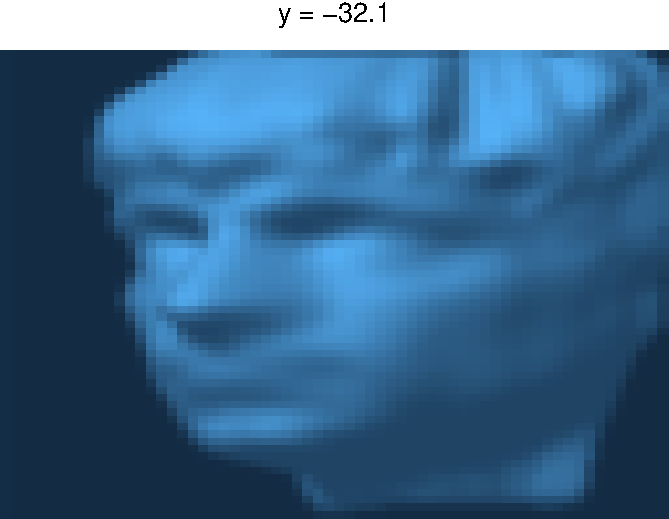
\includegraphics{SPAR_files/figure-pdf/unnamed-chunk-4-1.pdf}

We can split the data into training vs test sample:

\begin{verbatim}
set.seed(1234)
ntot <- length(y)
ntest <- ntot * 0.25
testind <- sample(1:ntot, ntest, replace=FALSE)
xtrain <- as.matrix(x[-testind, ])
const_col_ind <- which(apply(xtrain,2,sd)<0.01)
if (length(const_col_ind)>0) {
  xtrain <- xtrain[,-const_col_ind]
}
ytrain <- y[-testind]
xtest <- as.matrix(x[testind, -const_col_ind])
ytest <- y[testind]
\end{verbatim}

We can now estimate the model on the training data:

\begin{verbatim}
library(SPAR)
spar_faces <- spar.cv(xtrain, ytrain,
                      family = gaussian("identity"),
                      nummods = c(5, 10, 20, 50),
                      type.measure = "mse")
\end{verbatim}

\begin{verbatim}
Warning: glmnet.fit: algorithm did not converge

Warning: glmnet.fit: algorithm did not converge

Warning: glmnet.fit: algorithm did not converge

Warning: glmnet.fit: algorithm did not converge

Warning: glmnet.fit: algorithm did not converge

Warning: glmnet.fit: algorithm did not converge

Warning: glmnet.fit: algorithm did not converge

Warning: glmnet.fit: algorithm did not converge

Warning: glmnet.fit: algorithm did not converge

Warning: glmnet.fit: algorithm did not converge

Warning: glmnet.fit: algorithm did not converge

Warning: glmnet.fit: algorithm did not converge

Warning: glmnet.fit: algorithm did not converge

Warning: glmnet.fit: algorithm did not converge

Warning: glmnet.fit: algorithm did not converge

Warning: glmnet.fit: algorithm did not converge

Warning: glmnet.fit: algorithm did not converge

Warning: glmnet.fit: algorithm did not converge

Warning: glmnet.fit: algorithm did not converge

Warning: glmnet.fit: algorithm did not converge

Warning: glmnet.fit: algorithm did not converge

Warning: glmnet.fit: algorithm did not converge

Warning: glmnet.fit: algorithm did not converge

Warning: glmnet.fit: algorithm did not converge

Warning: glmnet.fit: algorithm did not converge

Warning: glmnet.fit: algorithm did not converge

Warning: glmnet.fit: algorithm did not converge

Warning: glmnet.fit: algorithm did not converge

Warning: glmnet.fit: algorithm did not converge

Warning: glmnet.fit: algorithm did not converge

Warning: glmnet.fit: algorithm did not converge

Warning: glmnet.fit: algorithm did not converge

Warning: glmnet.fit: algorithm did not converge

Warning: glmnet.fit: algorithm did not converge

Warning: glmnet.fit: algorithm did not converge

Warning: glmnet.fit: algorithm did not converge

Warning: glmnet.fit: algorithm did not converge

Warning: glmnet.fit: algorithm did not converge

Warning: glmnet.fit: algorithm did not converge

Warning: glmnet.fit: algorithm did not converge

Warning: glmnet.fit: algorithm did not converge

Warning: glmnet.fit: algorithm did not converge

Warning: glmnet.fit: algorithm did not converge

Warning: glmnet.fit: algorithm did not converge

Warning: glmnet.fit: algorithm did not converge

Warning: glmnet.fit: algorithm did not converge

Warning: glmnet.fit: algorithm did not converge

Warning: glmnet.fit: algorithm did not converge

Warning: glmnet.fit: algorithm did not converge

Warning: glmnet.fit: algorithm did not converge

Warning: glmnet.fit: algorithm did not converge

Warning: glmnet.fit: algorithm did not converge

Warning: glmnet.fit: algorithm did not converge

Warning: glmnet.fit: algorithm did not converge

Warning: glmnet.fit: algorithm did not converge

Warning: glmnet.fit: algorithm did not converge

Warning: glmnet.fit: algorithm did not converge

Warning: glmnet.fit: algorithm did not converge

Warning: glmnet.fit: algorithm did not converge

Warning: glmnet.fit: algorithm did not converge

Warning: glmnet.fit: algorithm did not converge

Warning: glmnet.fit: algorithm did not converge

Warning: glmnet.fit: algorithm did not converge

Warning: glmnet.fit: algorithm did not converge

Warning: glmnet.fit: algorithm did not converge

Warning: glmnet.fit: algorithm did not converge

Warning: glmnet.fit: algorithm did not converge

Warning: glmnet.fit: algorithm did not converge

Warning: glmnet.fit: algorithm did not converge

Warning: glmnet.fit: algorithm did not converge

Warning: glmnet.fit: algorithm did not converge

Warning: glmnet.fit: algorithm did not converge

Warning: glmnet.fit: algorithm did not converge

Warning: glmnet.fit: algorithm did not converge

Warning: glmnet.fit: algorithm did not converge

Warning: glmnet.fit: algorithm did not converge

Warning: glmnet.fit: algorithm did not converge

Warning: glmnet.fit: algorithm did not converge

Warning: glmnet.fit: algorithm did not converge

Warning: glmnet.fit: algorithm did not converge

Warning: glmnet.fit: algorithm did not converge

Warning: glmnet.fit: algorithm did not converge

Warning: glmnet.fit: algorithm did not converge

Warning: glmnet.fit: algorithm did not converge

Warning: glmnet.fit: algorithm did not converge

Warning: glmnet.fit: algorithm did not converge

Warning: glmnet.fit: algorithm did not converge

Warning: glmnet.fit: algorithm did not converge

Warning: glmnet.fit: algorithm did not converge

Warning: glmnet.fit: algorithm did not converge

Warning: glmnet.fit: algorithm did not converge

Warning: glmnet.fit: algorithm did not converge

Warning: glmnet.fit: algorithm did not converge

Warning: glmnet.fit: algorithm did not converge

Warning: glmnet.fit: algorithm did not converge

Warning: glmnet.fit: algorithm did not converge

Warning: glmnet.fit: algorithm did not converge

Warning: glmnet.fit: algorithm did not converge

Warning: glmnet.fit: algorithm did not converge

Warning: glmnet.fit: algorithm did not converge

Warning: glmnet.fit: algorithm did not converge

Warning: glmnet.fit: algorithm did not converge

Warning: glmnet.fit: algorithm did not converge

Warning: glmnet.fit: algorithm did not converge

Warning: glmnet.fit: algorithm did not converge

Warning: glmnet.fit: algorithm did not converge

Warning: glmnet.fit: algorithm did not converge

Warning: glmnet.fit: algorithm did not converge

Warning: glmnet.fit: algorithm did not converge

Warning: glmnet.fit: algorithm did not converge

Warning: glmnet.fit: algorithm did not converge

Warning: glmnet.fit: algorithm did not converge

Warning: glmnet.fit: algorithm did not converge

Warning: glmnet.fit: algorithm did not converge
\end{verbatim}

\begin{verbatim}
spar_faces
\end{verbatim}

\begin{verbatim}
SPAR.cv object:
Smallest CV-Meas 10.0 reached for nummod=50, lambda=0.000 leading to 3682 / 3833 active predictors.
Summary of those non-zero coefficients:
     Min.   1st Qu.    Median      Mean   3rd Qu.      Max. 
-33.85315  -0.14501   0.00034   0.01676   0.17048  36.39650 

Sparsest coefficient within one standard error of best CV-Meas reached for nummod=5, lambda=0.005 
leading to 1684 / 3833 active predictors with CV-Meas 14.6.
Summary of those non-zero coefficients:
     Min.   1st Qu.    Median      Mean   3rd Qu.      Max. 
-34.63019  -0.51653   0.04657   0.02366   0.58570  42.34801 
\end{verbatim}

\begin{verbatim}
# undebug(spar)
# 
# eig <- eigen(tcrossprod(z),symmetric = TRUE)
# myinv <- tcrossprod(eig$vectors[,eig$values>1e-8]%*%diag(1/sqrt(eig$values[eig$values>1e-8])))
# HOLP <- as.numeric(crossprod(z,myinv%*%yz))
# 
# n <- NROW(z)
# p <- NCOL(z)
# tmp_sc <- apply(z,2,function(col)sqrt(var(col)*(n-1)/n))
# z2 <- scale(z,center=colMeans(z),scale=tmp_sc)
# lam_max <- 1000 * max(abs(t(yz)%*%z2[,tmp_sc>0]))/n*family$mu.eta(family$linkfun(mean(yz)))/family$variance(mean(yz))
# dev.ratio_cutoff <- 0.999
# glmnet_res <- glmnet::glmnet(x=z, y=yz, family = family, alpha=0,lambda.min.ratio = min(0.01,1e-4 / lam_max))
# lam <- min(glmnet_res$lambda[glmnet_res$dev.ratio<=dev.ratio_cutoff])
# scr_coef <- coef(glmnet_res,s=lam)[-1]
# scr_coef
# 
# apply(glmnet_res$beta,2,function(tmpcoef)cor(tmpcoef,HOLP))
# 
# cor(scr_coef,HOLP)
\end{verbatim}

The \texttt{plot} method for `\texttt{spar.cv}' objects displays by
default the measure employed in the cross validation (in this case MSE)
for a grid of \(\lambda\) values, where the number of models is fixed to
the value found to perform best in cross-validation exercise:

\begin{verbatim}
plot(spar_faces)
\end{verbatim}

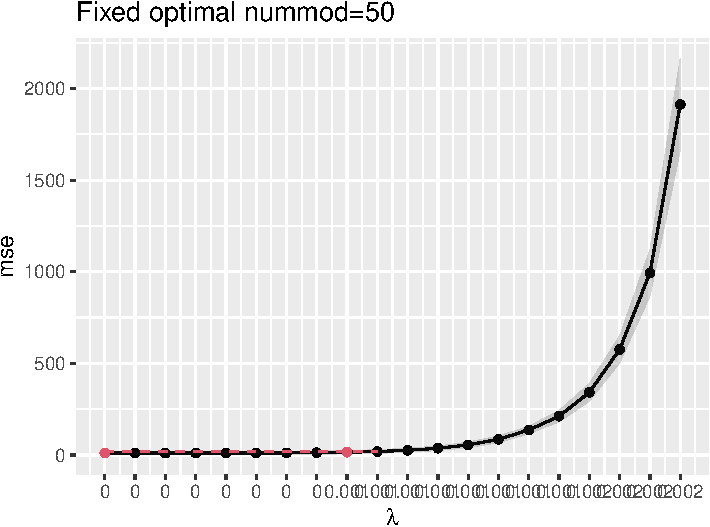
\includegraphics{SPAR_files/figure-pdf/unnamed-chunk-7-1.pdf}

\begin{verbatim}
# plot(spar_faces,plot_type = "Val_numAct")
\end{verbatim}

The coefficients of the different variables (in this example pixels)
obtained by averaging over the coefficients the marginal models (for
optimal \(\lambda\) and number of models) are given by:

\begin{verbatim}
face_coef <- coef(spar_faces, opt_par = "best")
str(face_coef)
\end{verbatim}

\begin{verbatim}
List of 4
 $ intercept: num -14.5
 $ beta     : num [1:3833] -0.63 -0.1982 0 -0.0989 1.0564 ...
 $ nummod   : num 50
 $ lambda   : num 0
\end{verbatim}

The coefficients from each of the marginal models (before averaging) can
be plotted using the \texttt{plot(...,\ plot\_type\ =\ "coefs")}

\begin{verbatim}
plot(spar_faces, "coefs")
\end{verbatim}

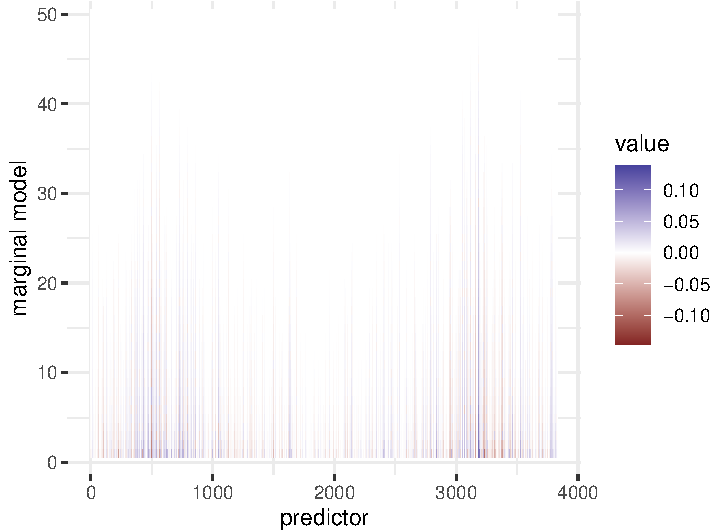
\includegraphics{SPAR_files/figure-pdf/unnamed-chunk-9-1.pdf}

The \texttt{predict()} function can be applied to the `\texttt{spar.cv}'
object:

\begin{verbatim}
ynew <- predict(spar_faces, xnew = xtest)
\end{verbatim}

In the high-dimensional setting it is interesting to look at the
relative mean square prediction error which compares the MSE to the MSE
of a model containing only an intercept:

\begin{verbatim}
rMSPEconst <- mean((ytest - mean(y))^2) 
mean((ynew-ytest)^2)/rMSPEconst
\end{verbatim}

\begin{verbatim}
[1] 0.01315477
\end{verbatim}

Additionally, for this data set, one can visualize the effect of each
pixel \(\hat\beta_j x^\text{new}_{i,j}\) in predicting the face
orientation in a given image e.g., 9th in the test set:

\begin{verbatim}
i <- 9
shap_vals <- numeric(64^2)
shap_vals[-const_col_ind] <- xtest[i,] * face_coef$beta
plot4 <- ggplot(data.frame(X = rep(1:64, each = 64),
                           Y = rep(64:1, 64),
                           effect = shap_vals), 
                aes(X, Y, fill= effect)) +
  geom_tile() +
  theme_void() +
  scale_fill_gradient2() +
  ggtitle(paste0("yhat=",round(ynew[i],2),", y=",round(ytest[i],2))) +
  theme(plot.title = element_text(hjust = 0.5)) 
plot4
\end{verbatim}

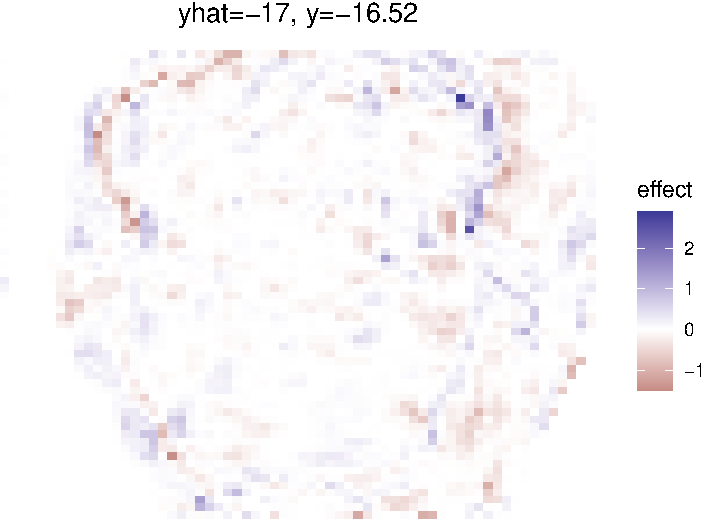
\includegraphics{SPAR_files/figure-pdf/unnamed-chunk-12-1.pdf}

\begin{verbatim}
# y[testind[i]]
# sum(xtest[i,] * face_coef$beta) + face_coef$intercept
\end{verbatim}

\subsection{Darwin data set}\label{darwin-data-set}

The Darwin dataset \citep{CILIA2022darwin} contains a binary response
for Alzheimer's disease (AD) together with extracted features from 25
handwriting tests (18 features per task) for 89 AD patients and 85
healthy people (\(n=174\)).

The data set can be downloaded from
https://archive.ics.uci.edu/dataset/732/darwin:

\begin{verbatim}
temp <- tempfile()
download.file("https://archive.ics.uci.edu/static/public/732/darwin.zip", temp)
darwin_tmp <- read.csv(unzip(temp,  "data.csv"), stringsAsFactors = TRUE)
\end{verbatim}

Before proceeding with the analysis, the data is screened for
multivariate outliers using the DDC algorithm in package \pkg{cellWise}.

\begin{verbatim}
darwin_orig <- list(
  x = as.matrix(darwin_tmp[, !(colnames(darwin_tmp) %in% c("ID", "class"))]),
  y = as.numeric(darwin_tmp$class) - 1)

tmp <- cellWise::DDC(darwin_orig$x,
                     list(returnBigXimp = TRUE, 
                          tolProb = 0.999,
                          silent = TRUE))
\end{verbatim}

\begin{verbatim}
 
 The final data set we will analyze has 174 rows and 446 columns.
 
\end{verbatim}

\begin{verbatim}
darwin <- list(x = tmp$Ximp,
               y = darwin_orig$y)
\end{verbatim}

We estimate the spar model with binomial family and logit link and use
\(1-\)area under the ROC curve as the cross-validation measure:

\begin{verbatim}
spar_darwin <- spar.cv(darwin$x, darwin$y,
                       family = binomial(logit),
                       nummods = c(5, 10, 20, 50),
                       type.measure = "1-auc")
\end{verbatim}

The \texttt{plot} method for `\texttt{spar.cv}' objects displays by
default the measure employed in the cross validation (in this case MSE)
for a grid of \(\lambda\) values, where the number of models is fixed to
the value found to perform best in cross-validation exercise:

\begin{verbatim}
plot(spar_darwin)
\end{verbatim}

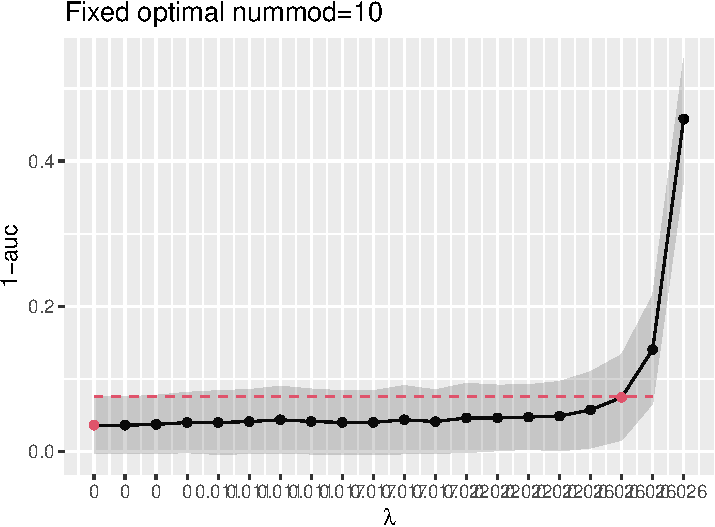
\includegraphics{SPAR_files/figure-pdf/unnamed-chunk-16-1.pdf}

The plot of the coefficients can be interpreted nicely in this example:

\begin{verbatim}
ntasks <- 25
nfeat <- 18
reorder_ind <- c(outer((seq_len(ntasks) - 1) * nfeat, seq_len(nfeat), "+"))
feat_names <- sapply(colnames(darwin$x)[seq_len(nfeat)],
                     function(name) substr(name, 1, nchar(name) - 1))

plot(spar_darwin,"coefs",coef_order = reorder_ind) + 
  geom_vline(xintercept = 0.5 + seq_len(ntasks - 1) * ntasks, 
             alpha = 0.2, linetype = 2) +
  annotate("text",x = (seq_len(nfeat) - 1) * ntasks + 12,
           y = 45,label=feat_names, angle = 90,
           size = 3)
\end{verbatim}

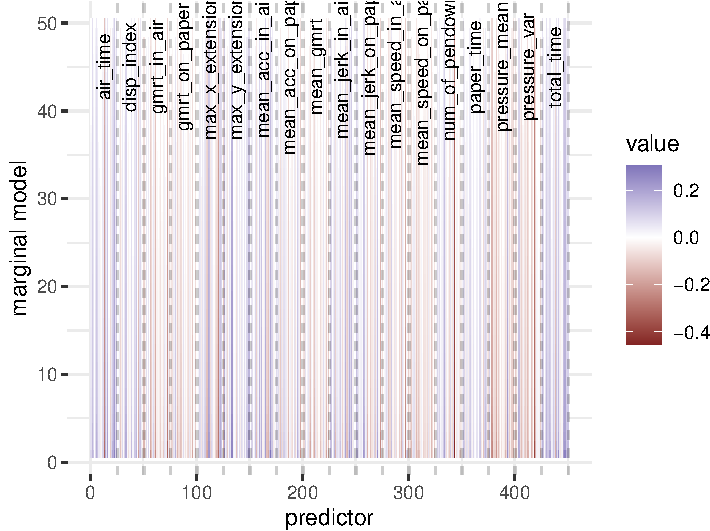
\includegraphics{SPAR_files/figure-pdf/unnamed-chunk-17-1.pdf}

In general we observe that the different features measures across
different tasks have the same impact on the probability of AD
(observable by the blocks of blue or red lines).

\section{Conclusion}\label{sec-conclusion}

Package \pkg{SPAR} provides an implementation for estimating an ensemble
of GLMs after performing probabilistic screening and random projection
in a high-dimensional setting.

\section*{Computational details}\label{computational-details}

The results in this paper were obtained using \proglang{R} 4.2.1.

\proglang{R} itself and all packages used are available from the
Comprehensive \proglang{R} Archive Network (CRAN) at
\url{https://CRAN.R-project.org/}.

\section*{Acknowledgments}\label{acknowledgments}

Roman Parzer and Laura Vana-Gür acknowledge funding from the Austrian
Science Fund (FWF) for the project ``High-dimensional statistical
learning: New methods to advance economic and sustainability policies''
(ZK 35), jointly carried out by WU Vienna University of Economics and
Business, Paris Lodron University Salzburg, TU Wien, and the Austrian
Institute of Economic Research (WIFO).


\renewcommand\refname{References}
  \bibliography{SPAR.bib}



\end{document}
